\documentclass[11pt]{article}

\def\asg{1}

\topmargin      -12ex
\textwidth	    165mm
\textheight	    244mm
\oddsidemargin	0mm
\evensidemargin	0mm

\usepackage{wrapfig}
\usepackage{xspace}
\usepackage{hyperref}
\usepackage{amsmath}
\usepackage{amssymb}
\usepackage{amsmath}
\usepackage{tikz}
\usepackage{fontspec}
\usepackage{unicode-math}
\usepackage{addfont}
\addfont{OT1}{seg-modified}{\seg}
\DeclareMathAlphabet{\mathcal}{OMS}{cmsy}{m}{n}

\newcommand{\false}{\ensuremath{\mathbf{f}}\xspace}
\newcommand{\true}{\ensuremath{\mathbf{t}}\xspace}
\newcommand{\impl}{\mathbin{\Rightarrow}}
\newcommand{\biim}{\mathbin{\Leftrightarrow}}

\newcounter{challenge}
\setcounter{challenge}{0}
\newcounter{task}
\setcounter{task}{0}

\renewcommand{\theequation}{\arabic{challenge}.\arabic{equation}}
\renewcommand{\thechallenge}{Challenge~\arabic{challenge}}
\newcommand{\challenge}[1]{
    \setcounter{task}{0}
    \setcounter{equation}{0}
    \refstepcounter{challenge}
    \section*{\thechallenge{} -- #1}
}
\renewcommand{\thetask}{Task~\arabic{challenge}\Alph{task}}
\newcommand{\task}{
    \refstepcounter{task}
    \paragraph{\thetask.}
}

\newcommand{\submission}[0]{\paragraph{Submission and Marking:}}
\newcommand{\pdfchallenges}[0]{\ref{ch:predicates} and \ref{ch:evenness}}
\newcommand{\pdfsubmission}[0]{
Your answers to \pdfchallenges{} should be submitted through
Gradescope as \emph{a single PDF document, no more than 2~MB in size}.
Marks are primarily allocated for correctness, 
but elegance and how clearly you communicate your thinking 
will also be taken into account.}
\newcommand{\groksubmission}[0]{
Your answer should be submitted on Grok.}
\newcommand{\simplegroksubmission}[0]{\groksubmission{}
You will find the submission format explained there.
You will receive some feedback from some elementary tests.
These merely check that your input has the correct format; 
they should not be relied upon for correctness. 
We will test your solution comprehensively after the deadline.}

\begin{document}

\begin{center}
    {\bf School of Computing and Information Systems \\ 
    COMP30026 Models of Computation}
    \bigskip \\
    {\Large\bf Assignment \asg}
    \bigskip \\
    {\large Released: 26 Aug. 2022; Deadline: 16 Sep. 2022}
\end{center}

\section*{Aims \& Procedure}

One aim of this assignment is to improve and test your understanding 
of propositional logic and first-order predicate logic,
including their use in mechanised reasoning.
A second aim is to develop your skills in analysis and 
formal reasoning about complex concepts,
and to practise writing down formal arguments with clarity.

This document is the assignment spec.
There are six challenges which you will find in the remainder of this document.
Your answers to \pdfchallenges{} are to be submitted through Gradescope,
for which there is a menu item on Canvas.
The remaining challenges are to be completed on Grok, 
where you will find a module called ``Assignment \asg''.
That module also contains more detailed information about 
submission formats and how to submit your answers in Grok. 

You are required to solve the challenges \emph{individually}.
You will probably find them to be of varying difficulty,
but each is worth 2~marks, for a total of 12.

\pagebreak

% Challenge 1
\challenge{Predictably Inconsistent Weather} \label{ch:logic-puzzle} 

\def\name{Harald}

The city of Melbourne, Australia is infamous for its predictably inconsistent weather.  
The mobile apps Parrot and Carrot compete to predict the correct weather over the next three days.  
Melbourne's weather has a habit of making a fool of the apps' developers, 
such that at any time, only one of the two apps makes a correct prediction.

Despite this, \name{} still can use this information to get accurate weather forecasts for the week, 
so that they don't get wet on their commutes to-and-from university.
On a Monday, \name{} checks both the Carrot and Parrot apps, where they make the following predictions:
\begin{align*}
    \text{Carrot:} &\quad \text{``It will rain on Tuesday and Wednesday.''}\\
    \text{Parrot:} &\quad \text{``If it rains on Monday, it will rain on Wednesday.''}
\end{align*}

\task \label{task:weather-formula} 
Capture, as a single propositional formula, the information that was thereby available to \name{}. 
You will need to take into account which app makes each prediction.  
Use propositional letters as follows:
\begin{gather*}
    C: \quad \text{Carrot's prediction is correct} \qquad  
    P: \quad \text{Parrot's prediction is correct}\\
    M: \quad \text{It rains on Monday}  \qquad 
    T: \quad \text{It rains on Tuesday} \qquad
    W: \quad \text{It rains on Wednesday}
\end{gather*}

\task \name{} tries to determine the weather forecast for the week from those two predictions, 
but realises they do not yet have enough information. 
Determine which truth assignments to $C, P, M, T, W$ make your formula from \ref{task:weather-formula} true.

\task \name{} opens their window blinds and looks outside to check for any chance of rain. 
Based on \textit{that} information, they now knew exactly what the weather would be for 
Monday, Tuesday and Wednesday.  Given this information, determine, for each of 
Monday, Tuesday and Wednesday, whether it rains or not.

\submission  

\simplegroksubmission{}
\ref{task:weather-formula} is worth 1 mark, the rest are worth 0.5 marks each.

\pagebreak

% Challenge 2
\challenge{Negative Implications} \label{ch:ands-and-nots} 

We have seen that implication can be re-written into an equivalent formula using the 
following equivalence
\begin{equation}
    \label{eq:impl-to-and-and-not} F \impl G\ \equiv\ \neg (F \land \neg G)
\end{equation}

In this challenge we will generalise this result to rewrite all of the connectives we
have seen using $\land$ and $\neg$.
To this effect, we will show that $\{\land, \neg\}$ is functionally complete as we can represent all
formulas using only $\land$ and $\neg$.

\task \label{task:re-write} 
Using the equivalence defined in \eqref{eq:impl-to-and-and-not}, re-write the following formula
to remove all instances of the $\impl$ connective. You \textbf{must not} perform any other transformations.

\begin{equation}
    \label{eq:implications} (\neg P \impl (\neg Q \land Q \impl \false))\ \impl\ (((P \impl \neg (R \impl Q)) \land \neg P)\ \impl\ \neg (P \impl \neg (R \impl Q))) 
\end{equation}

\task \label{task:simplify} 
The formula \eqref{eq:implications} can be simplified. Using \textbf{only} the equivalences
\eqref{eq:impl-to-and-and-not} and \eqref{eq:and-commutivity}--\eqref{eq:double-negation}
you can simplify your answer for \ref{task:re-write}. 
Provide the most simplified formula using \eqref{eq:impl-to-and-and-not} and
\eqref{eq:and-commutivity}--\eqref{eq:double-negation}, with \textbf{no} instances of $\impl$. 
This should contain the smallest number of connectives possible.

\begin{align}
    \label{eq:and-commutivity}     F \land G                &\ \equiv\ G \land F \\
    \label{eq:vacuous-conditional} \neg F \land (F \impl G) &\ \equiv\ \neg F \\
    \label{eq:double-negation}     \neg \neg F              &\ \equiv\ F
\end{align}

\task \label{task:re-write-all}
Generalising the re-writing rule \eqref{eq:impl-to-and-and-not}, 
we can re-write all other connectives using only $\land$ and $\neg$. 
Write a Haskell function that can re-write \textit{any} formula into an equivalent formula
that uses only $\land$, $\neg$, and any variables. 
Your function should \textbf{not} produce any double-negatives,
such as $\neg\neg P$.

\submission  

\simplegroksubmission{} 
\ref{task:re-write} and \ref{task:simplify} are worth 0.5 marks each for a correct answer;  
\ref{task:re-write-all} is worth 1 mark based proportionally on the number of passed
test cases.

\pagebreak

% Challenge 3
\challenge{Logic on Display} \label{ch:circuit}

\begin{wrapfigure}[10]{r}{0.2\textwidth}
\vspace*{-20pt}
\begin{center}
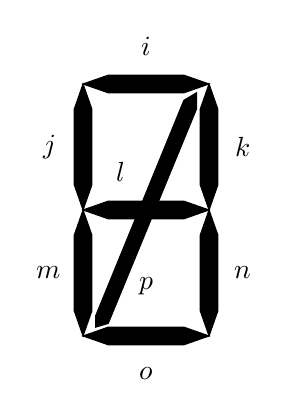
\begin{tikzpicture}
\begin{scope}[scale=0.16]

\path[draw,fill]% i
(-5,21)--(-3,21.7)--(3,21.7)--(5,21)--(3,20.3)--(-3,20.3)--cycle;
\path[draw,fill]% j
(-5,11)--(-4.3,13)--(-4.3,19)--(-5,21)--(-5.7,19)--(-5.7,13)--cycle;
\path[draw,fill]% k
(5,11)--(4.3,13)--(4.3,19)--(5,21)--(5.7,19)--(5.7,13)--cycle;
\path[draw,fill]% l
(-5,11)--(-3,11.7)--(3,11.7)--(5,11)--(3,10.3)--(-3,10.3)--cycle;
\path[draw,fill]% m
(-5,1)--(-4.3,3)--(-4.3,9)--(-5,11)--(-5.7,9)--(-5.7,3)--cycle;
\path[draw,fill]% n
(5,1)--(4.3,3)--(4.3,9)--(5,11)--(5.7,9)--(5.7,3)--cycle;
\path[draw,fill]% o
(-5,1)--(-3,1.7)--(3,1.7)--(5,1)--(3,0.3)--(-3,0.3)--cycle;
\path[draw,fill]% p
(3,19.7)--(4,20.3)--(4,19)--(-3,2)--(-4,1.7)--(-4,2.6)--cycle;

\node at (0,24)    {$i$};
\node at (-7.7,16) {$j$};
\node at (7.7,16)  {$k$};
\node at (-2,14)   {$l$};
\node at (-7.7,6)  {$m$};
\node at (7.7,6)   {$n$};
\node at (0,-2)    {$o$};
\node at (0,5)     {$p$};

\end{scope}
\end{tikzpicture}
\end{center}
\end{wrapfigure}

In this challenge we will consider an unconventional 8-segment display 
which is like a 7-segment display, but has an additional diagonal
LED from the top-right to bottom-left of the display. 
Arrays of such displays are commonly used to display characters in 
remote controls, blood pressure monitors, dishwashers, and other devices.
We label each LED $i$--$p$, with $p$ being the diagonal segment,
as shown here. 

Each LED can be on or off, but in most applications, 
only a small number of on/off combinations are of interest
(such as the ten combinations that allow the display of a digit 
in the range 0--9).
In that case, the display can be controlled through a small number of
input wires with four wires providing $2^4$ input combinations,
enough to cover the ten different digits.

Here we are interested in using an 8-segment display for some Greek letters. 
We want it to be able to show eight different letters, namely
$\Alpha$, $\Beta$, $\Gamma$, $\Delta$, $\Epsilon$, $\Zeta$, $\Eta$, and $\Lambda$.
For example, to show $\Alpha$, all the display segments, except $o$ and $p$,
should be lit up, giving the pattern {\seg A}.
In detail, we want the eight different letters displayed respectively as:
\begin{center}
{\Huge\seg A, B, C, D, E, F, H, L}
\end{center}
Since there are eight letters, we need three input wires, modelled as
propositional variables $P$, $Q$, and $R$.
We will need to decide on a suitable encoding of the eight letters.
One possibility encoding of the eight letters is to let $A$ correspond to input 000
(that is, $P = Q = R = \false$), $B$ to 001 
(that is, $P = Q = \false$ and $R = \true$), \textit{etc}.
If we do that, we can summarise the behaviour of each input
combination in the table below:
\begin{center}
\begin{tabular}{c|ccc|cccccccc|c}
    letter & $P$ & $Q$ & $R$ & $i$ & $j$ & $k$ & $l$ & $m$ & $n$ & $o$ & $p$ & display \\
\hline \hline
    $\Alpha$   & 0 & 0 & 0 & 1 & 1 & 1 & 1 & 1 & 1 & 0 & 0 & {\seg A} \\
    $\Beta$    & 0 & 0 & 1 & 1 & 1 & 1 & 1 & 1 & 1 & 1 & 0 & {\seg B} \\
    $\Gamma$   & 0 & 1 & 0 & 1 & 1 & 0 & 0 & 1 & 0 & 0 & 0 & {\seg C} \\
    $\Delta$   & 0 & 1 & 1 & 0 & 0 & 1 & 0 & 0 & 1 & 1 & 1 & {\seg D} \\
    $\Epsilon$ & 1 & 0 & 0 & 1 & 1 & 0 & 1 & 1 & 0 & 1 & 0 & {\seg E} \\
    $\Zeta$    & 1 & 0 & 1 & 1 & 0 & 0 & 0 & 0 & 0 & 1 & 1 & {\seg F} \\ 
    $\Eta$     & 1 & 1 & 0 & 0 & 1 & 1 & 1 & 1 & 1 & 0 & 0 & {\seg H} \\
    $\Lambda$  & 1 & 1 & 1 & 0 & 0 & 1 & 0 & 0 & 1 & 0 & 1 & {\seg L} \\
\end{tabular}
\end{center}
Each of the eight segments $i$--$p$ can be considered a propositional
function of the variables $P$, $Q$, and $R$.
This kind of display can be physically implemented with logic circuitry,
using circuits to implement a Boolean function for each of the outputs.
Here we assume that only three types of logic gates are available:
An \emph{and-gate} takes two inputs and produces, as output, the
conjunction ($\land$) of the inputs.
Similarly, an \emph{or-gate} implements disjunction ($\lor$).
Finally, an \emph{inverter} takes a single input and negates it ($\neg$).
We can specify such a circuit by writing down the Boolean equations
for each of the outputs $i$--$p$.
For example, segment $i$ is turned off (is false) when the
input is 011, 110, or, 111. 
So, $i$ can be captured as 
$(P \lor \neg Q \lor \neg R) 
\land (\neg P \lor \neg Q \lor R) 
\land (\neg P \lor \neg Q \lor \neg R)$.

For efficiency reasons, we often want the circuit to \emph{use as few gates
as possible}.
For example, the above equation for $i$ shows that we can implement this
output using fifteen gates. \linebreak
But 
$i = \neg (\neg P \land Q \land R) 
\land \neg (P \land Q \land \neg R) 
\land \neg (P \land Q \land R)$ is an equivalent implementation, 
using fewer gates.
Moreover, the eight functions might be able to \emph{share some circuitry}.
For example, if we have already implemented a sub-circuit defined by
$u = Q \land R$ (introducing $u$ as a name for the sub-circuit), then we
can define 
$i = \neg (\neg P \land u) 
\land \neg (P \land Q \land \neg R) 
\land \neg (P \land u)$, 
and we may be able to re-use $u$ while
implementing the other outputs (rather than duplicating the same gates).
In some cases, it may even be feasible to design a circuit 
that is not minimal for a given function, 
but provides a minimal solution when all eight functions are designed.

\task

Design such a circuit, using as few gates as possible.
You can define any number of sub-circuits to help you reduce the
gate count (simply give each a name).

\submission 

\groksubmission{}
Submit a text file \verb!circuit.txt! consisting of one line per definition.
This file will be tested automatically, 
so it is important that you follow the notational conventions exactly.
We write $\neg$ as \texttt{-} and $\lor$ as \texttt{+}.
We write $\land$ as \texttt{.}, or, more simply, we just leave it out,
so that concatenation of expressions denotes their conjunction.
Here is an example set of equations (for a different problem):
\begin{verbatim}
    # An example of a set of equations in the correct format:
    i = -Q R + Q -R + P -Q -R
    j = u + P (Q + R)
    k = P + -(Q R)
    l = u + P i
    u = -P -Q
    # u is an auxiliary function introduced to simplify j and l
\end{verbatim}

Empty lines, and lines that start with `\texttt{\#}', are ignored.
Input variables are in upper case.
Negation binds tighter than conjunction, which in
turn binds tighter than disjunction.
So the equation for $i$ says that
$i = (\neg Q \land R) \lor (Q \land \neg R)
        \lor (P \land \neg Q \land \neg R)$.
Note the use of a helper function $u$, allowing $j$ and $l$ to
share some circuitry.
Also note that we do not allow any feedback loops in the circuit.
In the example above, $l$ depends on $i$, so $i$ is not allowed
to depend, directly or indirectly, on $l$ (and indeed it does not).

To test your equations and count the number of gates used, you can click
{\bf\emph{Terminal}}
and enter the command \texttt{test}. To stop the {\bf\emph{Terminal}}, click {\bf\emph{Stop}}. 

There is one mark for a correct solution. 
An additional 0.5 is awarded if a correct solution uses 26 gates or fewer.
A further 0.5 is awarded if a correct solution uses 20 gates or fewer.

Optionally, you can submit your circuit design to a leaderboard. 
Your position on this board is not reflective of your final grade and can be used anonymously.
The leaderboard site can be found here \url{https://comp30026.ddns.net/leaderboard}.

\pagebreak

% Challenge 4
\challenge{Property-Based Testing} \label{ch:property-based-testing} 
Unlike unit tests that only test a single use case of a program, 
Property-Based Testing allows programmers to provide a specification of their programs, 
as logical properties that should hold if their program is implemented correctly. 
There are two types of properties that one can test about their code. 
One is data invariants which are light sanity checks and the others are full functional 
specifications.

For example, consider the following definition of \texttt{reverse} in Haskell
\begin{verbatim}
    reverse :: [a] -> [a]
    reverse []     = []
    reverse (x:xs) = reverse xs ++ [x]
\end{verbatim}

A nice property of a \texttt{reverse} function is that when composed with itself, it is the identity.
That is, to say
\begin{equation}
    \label{eq:rev-rev} \forall a\ \texttt{reverse}\ (\texttt{reverse}\ a)\ =\ a
\end{equation}

This property is not enough to show that the \texttt{reverse} is functionally correct, so we say that this is
a data invariant of \texttt{reverse}. For example, consider we replaced the definition of \texttt{reverse}
with \texttt{id} (the identity function), the property \eqref{eq:rev-rev} still holds.

For a full specification of the \texttt{reverse} function, we require a stronger property as follows
\begin{equation}
\begin{aligned}
    \forall a& \ \texttt{length}\ (\texttt{reverse}\ a)\ =\ \texttt{length}\ a \\ 
    & \quad\ \land\ \forall i\ 0 \leq i < \texttt{length}\ a\ \impl\ \texttt{reverse}\ a\ \texttt{!!}\ i\ =\ a\ \texttt{!!}\ (\texttt{length}\ a - i - 1) \\
\end{aligned}
\end{equation}

This specifies that the length of the reversal of some list, $a$, is the same as the length of $a$, 
and for each value of the reversal of some list, $a$, at index $i$, 
the value in $a$ at the opposing end of $a$ must be the same as said value in the reversal of $a$.
Take a moment to convince yourself this is true for a correct implementation of \texttt{reverse} and some 
example lists $a$.

In Haskell, the \textit{QuickCheck} library\footnote{\url{https://hackage.haskell.org/package/QuickCheck}}
provides property-based testing. This library is probably older 
than many of you, appearing first in 1999, and has been ported to well over 30 languages. 
In summary, QuickCheck generates a series of randomised inputs that are tested against the 
properties similar to the properties we have previously seen. QuickCheck then reports any 
test cases that fail as \textit{counter-examples}.
\textbf{You do not need to learn or understand QuickCheck to solve this challenge.}

Through this challenge, we will use a simplified model of property-based testing in Haskell.
We are concerned with the functional correctness of \textit{sorting functions}. To begin, we will be 
considering the following \textit{merge sort}, \texttt{msort}.
            
\begin{verbatim}
    msort :: (Ord a) => [a] -> [a]
    msort xs@(_:_:_) = msort (take n xs) `merge` msort (drop n xs)
      where n = length xs `div` 2
            merge [] rs = rs
            merge ls [] = ls
            merge lls@(l:ls) rrs@(r:rs) 
                | l < r     = l:merge ls  rrs
                | otherwise = r:merge lls rs
    msort xs = xs
\end{verbatim}

As we may have multiple sorting functions to test, the functions we will implement to test for these
properties we will see will parameterise which sorting function is to be tested, 
and so will have the following form

\begin{verbatim}
    sortProperty :: (Ord a) => ([a] -> [a]) -> [a] -> Bool
    sortProperty sort input = {- Boolean expression -} 
\end{verbatim}

Testing individual sorting functions is then performed with \texttt{sortProperty~msort}, \textit{etc.}

\task \label{task:sortLength}
Implement a function, \texttt{sortLength}, that checks the following property:
\textit{the result of sorting some input must have the same length as the input}.

\task \label{task:sortHead}
Implement a function, \texttt{sortHead}, that checks the following property:
\textit{if the input is not empty, then the head element of the sorted input is the least element of the input}.

\task \label{task:sortIsSorted}
Implement a function, \texttt{sortIsSorted}, that checks the following property:
\textit{the result of sorting some input is in sort-order, i.e., the result is a non-decreasing list}.

\task \label{task:sortSpec}
The following is a \textit{functional specification}
of all sorting functions:

\begin{verbatim}
    sortSpec :: (Ord a) => ([a] -> [a]) -> [a] -> Bool
    sortSpec sort input = 
        elem (sort input) (permutations input) && sortIsSorted sort input
\end{verbatim}

That is to say, a function sorts its input if the output is a permutation of 
the input and the output is in sort-order.\footnote{
\textit{Note:} this specification depends on the definition of the property from 
\ref{task:sortIsSorted} that you must implement yourself.}

With the following (incorrect) implementation of \texttt{qsort}, provide two values, 
\texttt{example} and \texttt{counterExample}, that are an example and a counter-example, 
respectively, for the \texttt{sortSpec} functional specification with respect to the \texttt{qsort} function.

\begin{verbatim}
    qsort :: (Ord a) => [a] -> [a]
    qsort [] = []
    qsort (pivot:rest) = qsort lesser ++ [pivot] ++ qsort greater
      where lesser  = filter (< pivot) rest
            greater = filter (> pivot) rest
\end{verbatim}

That is, \texttt{sortSpec~qsort~example} should be \texttt{True} and
\texttt{sortSpec~qsort~counterExample} should be \texttt{False}. 

\submission 

\simplegroksubmission{} Your functions should hold only for the properties asked. 
Each of \ref{task:sortLength}, \ref{task:sortHead}, and \ref{task:sortIsSorted} are worth 0.5 marks, 
each based proportionally on the number of test cases passed. 
\ref{task:sortSpec} is worth 0.5 marks, with 0.25 marks awarded for each correct value provided.

\pagebreak

% Challenge 5
\challenge{Interpreting Resolutions} \label{ch:predicates}

Consider the following predicate logic formulas.
\begin{align*}
    F: & \quad (\forall x \ Q(x)) \lor \exists x ((\forall y \ R(y,x) \lor Q(x)) \impl \exists z \forall y \ P(z,y)) \\
    G: & \quad \exists x \forall y \ (P(x,y) \lor (\exists z \ R(y,z) \impl \forall w \ Q(w))) \\
\end{align*}

\task Show that $F$ is non-valid, by providing an appropriate interpretation $\mathcal{I}$.
    
\task Show that $F \lor \neg G$ is valid using resolution, explicitly stating all substitutions used. 

\submission 

\pdfsubmission{}
The process of resolution should be displayed as a tree.

\pagebreak

% Challenge 6
\challenge{Evenness} \label{ch:evenness}

The notation we use for first-order predicate logic includes function symbols. 
This allows a very simple representation of the natural numbers. Namely, for natural numbers, 
we use terms built from a constant symbol (here we choose $a$, but any other symbol would do) 
and a one-place function symbol (we will use $s$, for ``successor''). 
The idea is that 0 is represented by $a$, 1 by $s(a)$, 2 by $s(s(a))$, and so on. 
In general, $s(x)$ represents the successor of $x$, that is, $x+1$. 
Logicians prefer this ``successor'' notation, because it uses so few symbols and 
supports recursive definition-—a natural number is either `$a$' (the base case), 
or it is of the form `$s(x)$', where $x$ is a term representing a natural number. 
(Of course, for practical use, we prefer the positional decimal system.)

With successor notation, we can capture addition by introducing a predicate symbol 
for the addition relation, letting $P(x, y, z)$ stand for $x + y = z$:
\begin{align}
    \label{eq:zero}    & \forall x \ P(a, x, x) && \text{(Identity element)}  \\
    \label{eq:add-one} & \forall x \forall y \forall z \ (P(x, y, z) \impl P(s(x), y, s(z)) && \text{(Recursive relation)} \\
    \label{eq:swap}    & \forall x \forall y \ (P(x, y, z) \impl P(y, x, z)) && \text{(Commutativity)}
\end{align}

Similarly, using the addition relation we can now define the evenness of a number by 
introducing the predicate symbol for evenness, letting $E(x)$ stand for $x$ \textit{is even}:
\begin{align}
    \label{eq:even-1} & \forall x \exists y \ (E(x) \impl P(y, y, x)) \\
    \label{eq:even-2} & \forall x \forall y \ (P(y, y, x) \impl E(x)) 
\end{align}

\task

Now, the goal is to prove the well-known property of natural numbers that if $n$ is an even number 
then $n+2$ is also even. Use resolution to show that 
\begin{equation}
    \label{eq:double-succ} \forall x \ (E(x) \impl E(s(s(x)))) 
\end{equation}
is a logical consequence of the axioms \eqref{eq:zero}--\eqref{eq:even-2}. 

\task

We have defined what an even number is and a theorem about even numbers, 
but we still don't know if even numbers exist! Using resolution, show that
\begin{equation*}
    \label{eq:triple-succ} \exists x \ E(s(s(s(x))))
\end{equation*}
is a logical consequence of the axioms \eqref{eq:zero}--\eqref{eq:even-2} and the theorem \eqref{eq:double-succ}. 
The resolution proof provides a sequence of most general unifiers, one per resolution step, 
and when these are composed in the order they were generated, you have a substitution that 
solves the constraint $E(s(s(s(x))))$. Give that substitution and explain what it means in 
terms of natural numbers.

\submission 

\pdfsubmission{}
The process of resolution should be displayed as a tree. 

\pagebreak

\subsection*{Further Submission Advice}

The deadline is 16 September at 23:00. Late submission will be possible, but a late submission
penalty will apply: a flagfall of 1 mark, and then 1 mark per 12 hours late.

Note that on Grok, ``saving'' your file does not mean submitting it for marking. To submit,
you need to click Mark and then Submit. You can submit as many times as you like. What gets
marked is the last submission you have made before the deadline.

For \pdfchallenges, if you produce an MS Word document, 
it must be exported and submitted as PDF, and satisfy the space limit of 2 MB. 
We also accept neat hand-written submissions, but these must be scanned and provided as PDF. 
Illegible or poorly-written submission will likely attract few, if any, marks.
If you scan your document, make sure you set the resolution so that the generated document 
is no more than 2 MB. The Canvas module, from which you downloaded this document, 
has advice to help you satisfy the 2~MB requirement while maintaining readability.

Being neat is easier if you type-set your answers, but not all typesetting software does a good
job of presenting mathematical formulas. The best tool is \LaTeX{}, which is worth learning if you
expect that you will later have to produce large technical documents. Admittedly, diagrams are
tedious to do with \LaTeX{}, even when using sophisticated packages such as Ti\textit{k}Z. You could, of
course, mix typeset text with hand-drawn diagrams. In case you want to use this assignment to
get some \LaTeX{} practice, we will leave the source for this document in the Canvas module where
you find the PDF version.

Make sure that you have enough time towards the end of the assignment to present your solutions
carefully. A nice presentation is sometimes more time consuming than solving the problems. Start
early; note that time you put in early usually turns out more productive than a last-minute effort.
For \ref{ch:circuit} in particular, you don’t want to submit some ``improved'' solution a few minutes
before the deadline, as it may turn out to be wrong and you won’t have time to change your mind.

\subsection*{Academic Honesty Statement}

By submitting work for assessment you implicitly declare that you 
understand the University’s policy on \textit{\textbf{academic integrity}} 
and that the work submitted is your original work. 
You declare that you have not been unduly assisted by any other person 
(collusion). 
In this assignment, \textit{\textbf{individual work}} is called for, 
but \textit{\textbf{if you get stuck}}, you can use the Ed Discussion 
board to ask any questions you have. 
As long as nobody directly gives away solutions, 
our discussion forum is both useful and appropriate for this; 
we can all use it to support each other's learning. 
If your question is simply to clarify some aspect of the assignment, 
your post can be `public', but if it reveals anything about your 
attempted solution, make sure it is submitted as a `private' post 
to the teaching team. 
Soliciting help from sources other than the above will be considered 
cheating and will lead to disciplinary action.

\end{document}